% Vista preliminar del código fuente

%% LyX 2.0.0 created this file.  For more info, see http://www.lyx.org/.
%% Do not edit unless you really know what you are doing.
\documentclass[english]{article}
\usepackage[T1]{fontenc}
\usepackage[latin9]{inputenc}
\usepackage[a4paper]{geometry}
\geometry{verbose,tmargin=2cm,bmargin=3cm,lmargin=2cm,rmargin=2cm}
\usepackage{array}
\usepackage{float}
\usepackage{multirow}
\usepackage{graphicx}

\makeatletter

%%%%%%%%%%%%%%%%%%%%%%%%%%%%%% LyX specific LaTeX commands.
%% Because html converters don't know tabularnewline
\providecommand{\tabularnewline}{\\}

%%%%%%%%%%%%%%%%%%%%%%%%%%%%%% Textclass specific LaTeX commands.
\newenvironment{lyxcode}
{\par\begin{list}{}{
\setlength{\rightmargin}{\leftmargin}
\setlength{\listparindent}{0pt}% needed for AMS classes
\raggedright
\setlength{\itemsep}{0pt}
\setlength{\parsep}{0pt}
\normalfont\ttfamily}%
 \item[]}
{\end{list}}

\makeatother

\usepackage{babel}
\begin{document}

\title{Aprendizaje Automático - Trabajo Práctico 4}


\author{Gonzalo Castiglione - 49138}

\maketitle

\paragraph*{Objetivo: Aprender a agrupar datos mediante análisis de clusters}


\section{Determinación de clases. Clustering.}
\begin{enumerate}
\item (TO DO)
\item Lirios de Fisher

\begin{enumerate}
\item Clasificación del las mediciónes según el algoritmo $kmeans$


\begin{center}
\begin{figure}[H]
\begin{centering}
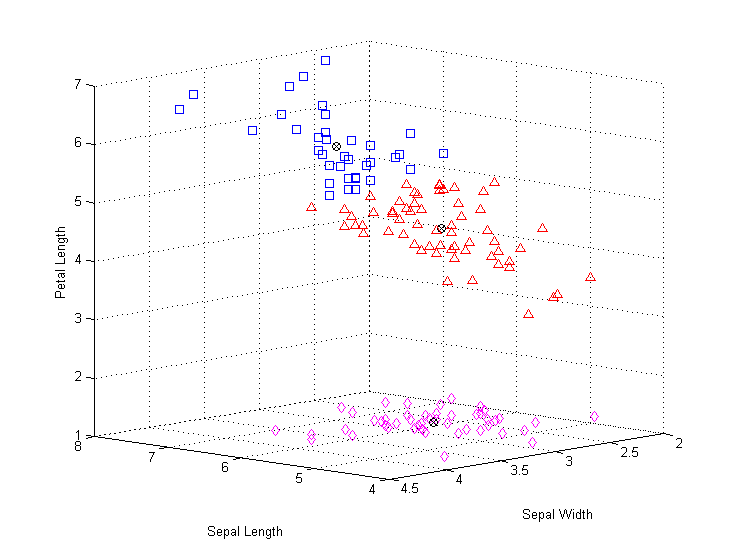
\includegraphics[scale=0.5]{kmeans2}\caption{Agrupamiento de los lirios de Fisher}

\par\end{centering}

\end{figure}

\par\end{center}


Matriz de confusión


\begin{center}
\begin{tabular}{|c|c|c|c|c|}
\hline 
 & \multicolumn{4}{c|}{Clase Predicha}\tabularnewline
\hline 
\multirow{4}{*}{Clase Real} &  & Setosa & Versicolor & Virginica\tabularnewline
\cline{2-5} 
 & Setosa & $50$ & $0$ & $0$\tabularnewline
\cline{2-5} 
 & Versicolor & $0$ & $42$ & $8$\tabularnewline
\cline{2-5} 
 & Virginica & $0$ & $14$ & $36$\tabularnewline
\hline 
\end{tabular}
\par\end{center}

\item Calsificación 


\begin{center}
\begin{figure}[H]
\centering{}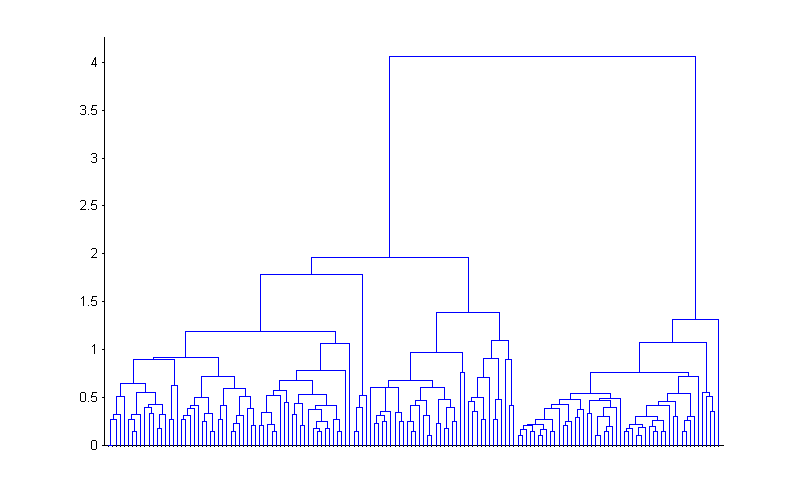
\includegraphics[scale=0.5]{dendograma}\caption{Agrupamiento de los lirios de Fisher}
\end{figure}

\par\end{center}


Matriz de confusión


\begin{center}
\begin{tabular}{|c|c|c|c|c|}
\hline 
 & \multicolumn{4}{c|}{Clase Predicha}\tabularnewline
\hline 
\multirow{4}{*}{Clase Real} &  & Setosa & Versicolor & Virginica\tabularnewline
\cline{2-5} 
 & Setosa & $50$ & $0$ & $0$\tabularnewline
\cline{2-5} 
 & Versicolor & $0$ & $49$ & $1$\tabularnewline
\cline{2-5} 
 & Virginica & $0$ & $15$ & $35$\tabularnewline
\hline 
\end{tabular}
\par\end{center}

\end{enumerate}
\end{enumerate}
\newpage{}


\section{Código}
\begin{enumerate}
\item (TO DO)
\item Lirios de Fisher

\begin{lyxcode}
//~a)

ptsymb~=~\{'bs','r\textasciicircum{}','md','go','c+'\};

load~fisheriris;

k~=~3;

{[}cidx,cmeans,sumd{]}~=~kmeans(meas,k);

for~i~=~1:k
\begin{lyxcode}
clust~=~find(cidx==i);

plot3(meas(clust,1),~meas(clust,2),~meas(clust,3),~ptsymb\{i\});

hold~on
\end{lyxcode}
end~

plot3(cmeans(:,1),~cmeans(:,2),~cmeans(:,3),'ko');~

plot3(cmeans(:,1),~cmeans(:,2),~cmeans(:,3),'kx');

hold~off

xlabel('Sepal~Length');

ylabel('Sepal~Width');

zlabel('Petal~Length');

view(-137,10);

grid~on



types~=~{[}ones(1,50){*}2~ones(1,50)~ones(1,50){*}3{]};

cMat~=~confusionmat(types,cidx)



//~b)

eucD~=~pdist(meas,~'euclidean');

clustTreeEuc~=~linkage(eucD,~'average');

{[}h,~nodes{]}~=~dendrogram(clustTreeEuc,~0);

set(gca,~'TickDir',~'out',~'TickLength',~{[}.002~0{]},~'XTickLabel',~{[}{]});



dist~=~pdist(~data~);~

linkage\_matrix~=~linkage(~dist,~\textquoteleft{}ward'~);~

cluster\_labels~=~cluster(~linkage\_matrix,~'maxclust',~3~);~

confusion\_matrix~=~crosstab(~cluster\_labels,~class~)~
\end{lyxcode}
\end{enumerate}
\begin{lyxcode}
\end{lyxcode}

\end{document}
